% =====================================================================
%  Proyecto Aprendizaje por Refuerzo - Cuarto 8x8 con obstáculos móviles
%  Definición de estados, acciones y recompensas
%  Compilar con pdfLaTeX:  latexmk -pdf definicion_ambiente.tex
%  Cada tripla (s,a,s') de la sección 4 está verificada en tests/test_gridworld.py
% =====================================================================
\documentclass[11pt,letterpaper]{article}

\usepackage[T1]{fontenc}
\usepackage[utf8]{inputenc}
\usepackage{babel}
\babelprovide[import,main]{spanish}
\usepackage{lmodern}
\usepackage[margin=2.3cm]{geometry}
\usepackage{fancyhdr}
\usepackage{titlesec}
\usepackage{parskip}
\usepackage{amsmath,amssymb}
\usepackage{booktabs}
\usepackage{tabularx}
\usepackage{array}
\usepackage[table]{xcolor}
\usepackage{enumitem}
\usepackage{caption}
\usepackage{graphicx}
\usepackage{float}
\usepackage[colorlinks=true,linkcolor=azul,urlcolor=azul]{hyperref}

\definecolor{azul}{HTML}{1F4E79}
\titleformat{\section}{\Large\bfseries\color{azul}}{\thesection.}{0.6em}{}
\titleformat{\subsection}{\large\bfseries\color{azul}}{\thesubsection}{0.6em}{}
\captionsetup{font=small,labelfont=bf}
\setlist{itemsep=2pt,topsep=4pt}
\newcolumntype{L}{>{\raggedright\arraybackslash}X}
\newcolumntype{P}[1]{>{\raggedright\arraybackslash}p{#1}}
\renewcommand{\arraystretch}{1.25}
\setlength{\emergencystretch}{2em}
\graphicspath{{figuras/}}

\pagestyle{fancy}
\fancyhf{}
\lhead{\small Aprendizaje por Refuerzo -- Proyecto}
\rhead{\small Cuarto 8x8 con obstáculos móviles}
\cfoot{\small \thepage}

\newcommand{\IZQ}{\mathsf{GIRAR\_IZQ}}
\newcommand{\DER}{\mathsf{GIRAR\_DER}}
\newcommand{\AV}{\mathsf{AVANZAR}}
\newcommand{\META}{s_{\mathrm{META}}}
\newcommand{\COL}{s_{\mathrm{COL}}}
\newcommand{\code}[1]{\texttt{#1}}

\begin{document}

\begin{center}
  {\small Universidad de los Andes \textperiodcentered{} Maestría en Inteligencia Artificial}\\[2pt]
  {\small Aprendizaje por Refuerzo \textperiodcentered{} Prof. Nicolás Cardozo}\\[10pt]
  {\LARGE\bfseries\color{azul} Agente de RL en un cuarto 8x8\\[2pt] con obstáculos móviles}\\[8pt]
  {\large Definición de estados, acciones y función de recompensa}\\[8pt]
  Miguel Ángel Muñoz Layton \quad\textperiodcentered\quad Daniel F. Barrera Armendaris\\[2pt]
  {\small Noviembre de 2026}
\end{center}

\vspace{4pt}
\hrule
\vspace{8pt}

\section*{Correspondencia con la rúbrica}

\begin{table}[H]
\centering\small
\begin{tabularx}{\textwidth}{@{}P{2.4cm}P{1.5cm}L@{}}
\toprule
\textbf{Criterio} & \textbf{Sección} & \textbf{Qué se define} \\
\midrule
Estados & 2 & Estado completo del ambiente: posición $(f,c)$ y orientación $\theta$ del agente, posiciones de los cinco obstáculos, inicio $(0,0)$, meta $(7,7)$ y los estados terminales de llegada ($\META$) y colisión ($\COL$). Tipo, rango y restricciones de cada variable. Además, el estado $\phi(s)$ que usa la Q-tabla y por qué basta para aprender \\
Acciones & 3 & $\IZQ$ (girar $90^\circ$ a la izquierda), $\DER$ (girar $90^\circ$ a la derecha) y $\AV$ (moverse a la casilla de enfrente si existe), con $A(s)$ explícito para cada estado del tablero, su efecto y la dinámica simultánea de los obstáculos \\
Recompensas & 4 & $R(s,a,s')$ para todos los casos: llegar a $(7,7)$ ($+100$), chocar con un obstáculo ($-100$), costo de cada paso y de cada giro ($-1$), avance inválido ($-10$) y estados terminales. Diez triplas $(s,a,s')$ de ejemplo \\
\bottomrule
\end{tabularx}
\end{table}

% =====================================================================
\section{El ambiente}

El ambiente es un cuarto vacío de $8\times8$ casillas. El agente (triángulo negro) siempre empieza en la
casilla superior izquierda $(0,0)$ y su objetivo es llegar a la casilla inferior derecha $(7,7)$ (cuadrado
verde) sin estrellarse con ninguno de los cinco obstáculos (círculos azules). Los obstáculos aparecen en
posiciones aleatorias y en cada paso se mueven al azar, al mismo tiempo que el agente actúa. Si el agente
choca con un obstáculo, el episodio termina.

\begin{figure}[H]
\centering
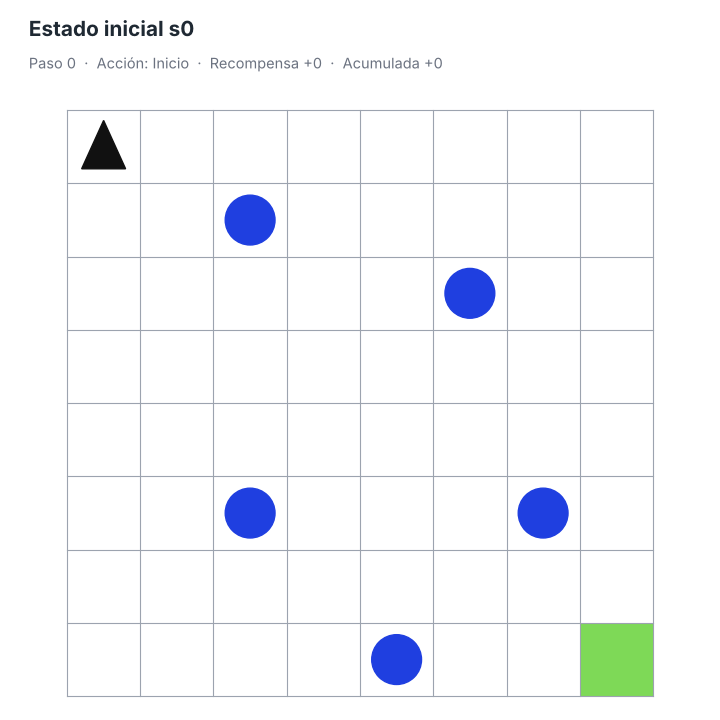
\includegraphics[width=0.42\textwidth]{estado_inicial.png}\hspace{0.04\textwidth}%
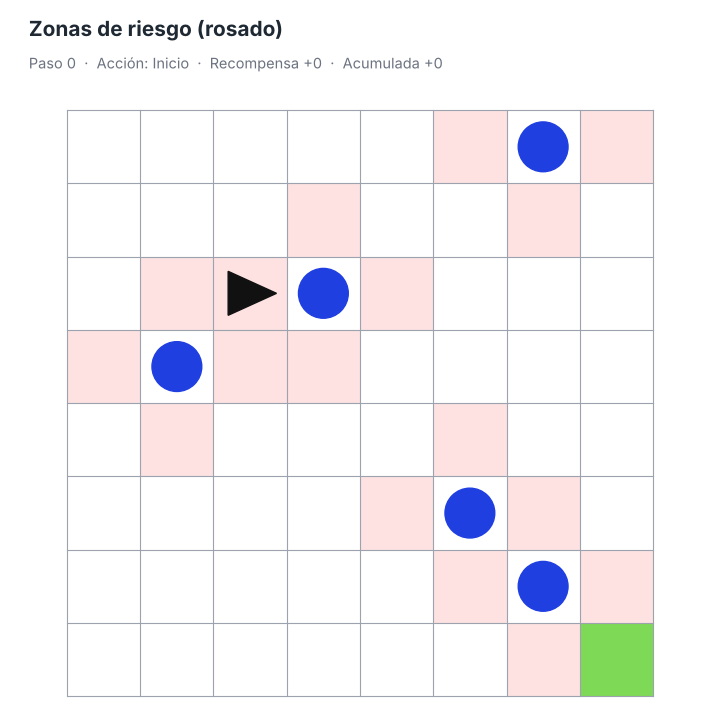
\includegraphics[width=0.42\textwidth]{percepcion.png}
\caption{Izquierda: un estado inicial (agente en $(0,0)$ mirando al norte, como en la figura del enunciado).
Derecha: las casillas en rosado son las que un obstáculo puede ocupar en el siguiente paso.}
\label{fig:tablero}
\end{figure}

\textbf{Convenciones.} Las casillas se indican como $(f,c)$, con fila $f$ y columna $c$ entre 0 y 7; $(0,0)$ es
la esquina superior izquierda y $(7,7)$ la inferior derecha. La orientación $\theta$ toma los valores
N (arriba, $f-1$), E (derecha, $c+1$), S (abajo, $f+1$) y O (izquierda, $c-1$). La casilla de enfrente es
$\mathrm{fr}(f,c,\theta)$; por ejemplo, $\mathrm{fr}(2,2,\mathrm{E})=(2,3)$.

\textbf{Dinámica de los obstáculos.} En cada paso, cada obstáculo elige al azar, con igual probabilidad, entre
quedarse en su casilla o moverse a una de sus cuatro vecinas, descartando las que están fuera del cuarto, la
meta $(7,7)$ o una casilla ya ocupada por otro obstáculo. Los obstáculos sí pueden entrar en la casilla del
agente: eso es una colisión. Así la meta nunca queda bloqueada y siempre existe un camino.

\textbf{Movimiento simultáneo y colisión.} El agente aplica su acción y los obstáculos se mueven en el mismo
paso. Hay colisión si, después del paso, (i) el agente y un obstáculo ocupan la misma casilla, o (ii) el agente
y un obstáculo intercambiaron casillas (se cruzaron). Girar no protege: si un obstáculo entra en la casilla del
agente mientras gira, también hay colisión.

% =====================================================================
\section{Conjunto de estados}

\subsection{Estado completo del ambiente}

Un estado no terminal es
\[
  s = (f,\ c,\ \theta,\ o_1,\ o_2,\ o_3,\ o_4,\ o_5),
\]
con las variables del cuadro~\ref{tab:estado}.

\begin{table}[H]
\centering\small
\begin{tabularx}{\textwidth}{@{}P{1.9cm}P{4.2cm}P{2.6cm}L@{}}
\toprule
\textbf{Variable} & \textbf{Descripción} & \textbf{Tipo y rango} & \textbf{Restricciones} \\
\midrule
$(f, c)$ & Posición del agente & Entero, $\{0,\dots,7\}^2$ & $(f,c)\neq(7,7)$ en un estado no terminal \\
$\theta$ & Orientación del agente & Categórica, $\{\mathrm{N},\mathrm{E},\mathrm{S},\mathrm{O}\}$ & Cambia solo al girar \\
$o_i=(f_i,c_i)$, $i=1..5$ & Posición de cada obstáculo & Entero, $\{0,\dots,7\}^2$ & Distintas entre sí, distintas de $(7,7)$ y de $(f,c)$ \\
\bottomrule
\end{tabularx}
\caption{Variables del estado completo.}
\label{tab:estado}
\end{table}

\begin{itemize}
  \item \textbf{Estado inicial} $s_0$: el agente en el inicio $(0,0)$ mirando al norte; los cinco obstáculos en
    casillas distintas elegidas al azar entre todas, excepto $(0,0)$ y $(7,7)$.
  \item \textbf{Meta}: la casilla $(7,7)$ es fija. Como los obstáculos tampoco cambian de número, los cinco
    siempre forman parte del estado.
  \item \textbf{Estados terminales}: $\META$ (el agente llegó a $(7,7)$ sin chocar) y $\COL$ (el agente chocó
    con un obstáculo). En ambos el episodio termina y no hay acciones.
  \item \textbf{Tamaño}: hay $63\cdot4\cdot\binom{62}{5}$, es decir $1\,630\,692\,504$, estados no terminales,
    más los 2 terminales. Los obstáculos son intercambiables, así que se cuentan como un conjunto.
  \item \textbf{Límite de pasos}: si el agente no termina en 200 pasos, el episodio se corta. Es un límite
    práctico de la simulación, no un estado terminal del MDP.
\end{itemize}

Este estado es de Markov: con la posición y la orientación del agente y las posiciones de los obstáculos, la
distribución del siguiente estado y de la recompensa depende solo de la acción. Los obstáculos se mueven sin
memoria y no dependen de pasos anteriores.

\subsection{Estado que usa la Q-tabla}

Una Q-tabla con 1\,600 millones de filas no se puede llenar: el agente casi nunca vería dos veces la misma
configuración de obstáculos. Por eso el agente aprende sobre una representación $\phi(s)$ calculada a partir
del estado completo. Conserva la posición y la orientación, y resume los obstáculos con lo que importa para
decidir:
\[
  \phi(s) = (f,\ c,\ \theta,\ \mathit{fr},\ \mathit{aq},\ \mathit{iz},\ \mathit{de}).
\]

\begin{table}[H]
\centering\small
\begin{tabularx}{\textwidth}{@{}P{1.6cm}P{2.6cm}L@{}}
\toprule
\textbf{Variable} & \textbf{Rango} & \textbf{Significado} \\
\midrule
$f, c, \theta$ & Como en el estado completo & Dónde está el agente y hacia dónde mira \\
$\mathit{fr}$ & $\{0,1,2,3\}$ & Casilla de enfrente: 0 libre, 1 en riesgo (un obstáculo está al lado y puede entrar en el siguiente paso), 2 ocupada por un obstáculo, 3 pared \\
$\mathit{aq}$ & $\{0,1\}$ & 1 si algún obstáculo está al lado del agente y puede entrar en su casilla \\
$\mathit{iz}$, $\mathit{de}$ & $\{0,1\}$ & 1 si la casilla a la izquierda (o derecha) del agente está ocupada o en riesgo \\
\bottomrule
\end{tabularx}
\caption{Estado tabular $\phi(s)$: $8\cdot8\cdot4\cdot4\cdot2\cdot2\cdot2=8\,192$ combinaciones.}
\end{table}

\textbf{Por qué basta para aprender.} Un obstáculo se mueve a lo sumo una casilla por paso. Por eso, en el
siguiente paso solo puede causar una colisión si está a una casilla del agente o de la casilla de enfrente:
entrando en la casilla del agente, entrando en la casilla a la que el agente avanza, o cruzándose con él.
Esos son justamente los casos que distinguen $\mathit{aq}$ y $\mathit{fr}$. Los otros obstáculos no pueden
afectar el resultado inmediato de ninguna acción. $\mathit{iz}$ y $\mathit{de}$ anticipan qué pasará después
de girar. La posición y la orientación le permiten aprender el camino hacia $(7,7)$. Lo que se pierde (cuántos
obstáculos hay y en qué dirección exacta) solo afecta la probabilidad de chocar, no la posibilidad de hacerlo.

% =====================================================================
\section{Acciones del agente}

$A = \{\IZQ,\ \DER,\ \AV\}$: los dos grados de libertad que define el enunciado, rotar sobre su eje y moverse
hacia adelante.

\begin{table}[H]
\centering\small
\begin{tabularx}{\textwidth}{@{}P{2.4cm}P{4.6cm}L@{}}
\toprule
\textbf{Acción} & \textbf{Efecto sobre el agente} & \textbf{Estados en los que se puede ejecutar} \\
\midrule
$\IZQ$ & Rota $90^\circ$ a la izquierda: $\mathrm{N}\to\mathrm{O}\to\mathrm{S}\to\mathrm{E}\to\mathrm{N}$. La posición no cambia & Todos los estados no terminales \\
$\DER$ & Rota $90^\circ$ a la derecha: $\mathrm{N}\to\mathrm{E}\to\mathrm{S}\to\mathrm{O}\to\mathrm{N}$. La posición no cambia & Todos los estados no terminales \\
$\AV$ & Pasa a la casilla de enfrente, $\mathrm{fr}(f,c,\theta)$; la orientación no cambia & Estados no terminales en los que la casilla de enfrente existe. No aplica si mira a una pared: $f=0$ y $\theta=\mathrm{N}$; $f=7$ y $\theta=\mathrm{S}$; $c=0$ y $\theta=\mathrm{O}$; $c=7$ y $\theta=\mathrm{E}$ \\
\bottomrule
\end{tabularx}
\caption{Acciones del agente.}
\end{table}

En resumen, $A(s)$ es:
\[
A(s)=\begin{cases}
\emptyset & \text{si } s\in\{\META,\COL\}\\[2pt]
\{\IZQ,\DER\} & \text{si } \mathrm{fr}(f,c,\theta)\ \text{está fuera del cuarto}\\[2pt]
A & \text{en cualquier otro caso.}
\end{cases}
\]
Por ejemplo, en el estado inicial (agente en $(0,0)$ mirando al norte) solo puede girar. Avanzar hacia una
casilla con un obstáculo sí está permitido, porque el obstáculo puede moverse en ese mismo paso; el riesgo se
refleja en la recompensa. En total hay 32 pares (casilla, orientación) del borde en los que $\AV$ no aplica.

\textbf{Transición.} Desde $s$ con la acción $a\in A(s)$: (1) el agente gira o avanza según el cuadro anterior;
(2) al mismo tiempo, cada obstáculo se mueve según la dinámica de la sección 1; (3) si hay colisión,
$s'=\COL$; si no y el agente está en $(7,7)$, $s'=\META$; si no, $s'$ es el nuevo estado no terminal. Como la
meta nunca tiene obstáculos, llegar a ella y chocar no pueden ocurrir a la vez.

% =====================================================================
\section{Función de recompensa \texorpdfstring{$R(s,a,s')$}{R(s,a,s')}}

\[
R(s,a,s')=\begin{cases}
+100 & \text{si } s'=\META \quad\text{(llegar a la meta)}\\
-100 & \text{si } s'=\COL \quad\text{(chocar con un obstáculo, con cualquier acción)}\\
-10 & \text{si } a=\AV \text{ contra una pared y } s'\ \text{no es terminal}\\
-1 & \text{en otro caso: cada paso y cada giro}
\end{cases}
\]

\begin{table}[H]
\centering\small
\begin{tabularx}{\textwidth}{@{}P{6.6cm}cL@{}}
\toprule
\textbf{Situación $(s,a,s')$} & \textbf{$R$} & \textbf{Justificación} \\
\midrule
Cualquier $a$ que lleva a $s'=\META$ & $+100$ & Es el objetivo. Supera el costo de cualquier camino razonable (el más corto tiene 14 avances y al menos 2 giros), así que llegar siempre conviene \\
Cualquier $a$ que lleva a $s'=\COL$ (avanzar hacia un obstáculo, cruzarse con él, o que un obstáculo entre mientras el agente gira) & $-100$ & Chocar es tan malo como bueno es llegar: el agente no gana nada arriesgándose a chocar para acortar camino \\
$a=\AV$ y $s'$ no terminal & $-1$ & Costo de cada paso: premia los caminos cortos \\
$a\in\{\IZQ,\DER\}$ y $s'$ no terminal & $-1$ & Costo de cada giro: girar consume un paso y lo deja expuesto, así que no puede girar en círculos gratis \\
$a=\AV$ contra una pared ($a\notin A(s)$), sin máscara & $-10$ & Solo aplica si una implementación no restringe a $A(s)$. El agente no se mueve, pero los obstáculos sí; si uno entra en su casilla, aplica $-100$ \\
$s\in\{\META,\COL\}$ & -- & Estado terminal: no hay acciones ni recompensas \\
\bottomrule
\end{tabularx}
\caption{Recompensas para todas las situaciones posibles.}
\end{table}

\textbf{Descuento y comportamiento esperado.} Se usa $\gamma=0{,}95$. Con estas recompensas, la política óptima
llega a $(7,7)$ por un camino corto, gira solo cuando hace falta y, cuando un obstáculo amenaza la casilla de
enfrente, prefiere esperar girando o desviarse antes que avanzar hacia él.

\subsection{Triplas \texorpdfstring{$(s,a,s')$}{(s,a,s')} de ejemplo}

Notación: $s=(f,c,\theta\,|\,o_1,\dots,o_5)$. Salvo que se indique otra cosa, los obstáculos están lejos:
$O=\{(4,4),(4,6),(6,2),(2,6),(3,3)\}$. Cada tripla está verificada con una prueba automática del código
(\code{tests/test\_gridworld.py}).

\begin{table}[H]
\centering\footnotesize
\setlength{\tabcolsep}{4pt}
\begin{tabularx}{\textwidth}{@{}P{0.6cm}P{3.3cm}P{2.2cm}P{3.1cm}Lc@{}}
\toprule
\textbf{\#} & \textbf{Estado $s$} & \textbf{Acción} & \textbf{Estado $s'$} & \textbf{Qué pasa} & \textbf{$R$} \\
\midrule
T1 & $(0,0,\mathrm{N}\,|\,O)$ & $\IZQ$ & $(0,0,\mathrm{O}\,|\,O')$ & Gira sin chocar & $-1$ \\
T2 & $(0,0,\mathrm{N}\,|\,O)$ & $\DER$ & $(0,0,\mathrm{E}\,|\,O')$ & Gira hacia el camino a la meta & $-1$ \\
T3 & $(0,0,\mathrm{E}\,|\,O)$ & $\AV$ & $(0,1,\mathrm{E}\,|\,O')$ & Avanza a una casilla libre & $-1$ \\
T4 & $(7,6,\mathrm{E}\,|\,O)$ & $\AV$ & $\META$ & Llega a $(7,7)$ & $+100$ \\
T5 & $(2,2,\mathrm{E}\,|\,(2,3),\dots)$ & $\AV$ & $\COL$ & El obstáculo de $(2,3)$ se queda: el agente entra en él & $-100$ \\
T6 & $(2,2,\mathrm{E}\,|\,(2,3),\dots)$ & $\AV$ & $\COL$ & El obstáculo pasa a $(2,2)$ mientras el agente pasa a $(2,3)$: se cruzan & $-100$ \\
T7 & $(2,2,\mathrm{N}\,|\,(3,2),\dots)$ & $\DER$ & $\COL$ & El obstáculo de $(3,2)$ entra en la casilla del agente mientras gira & $-100$ \\
T8 & $(0,0,\mathrm{N}\,|\,O)$ & $\AV$ (sin máscara) & $(0,0,\mathrm{N}\,|\,O')$ & Avanza contra la pared: no se mueve & $-10$ \\
T9 & $\META$ o $\COL$ & -- & -- & Terminal: $A(s)=\emptyset$ & -- \\
T10 & Paso 200 sin terminar & Cualquiera & No terminal & El episodio se corta por el límite; la recompensa es la de la acción & $-1$ \\
\bottomrule
\end{tabularx}
\caption{Ejemplos de $R(s,a,s')$. $O'$ son las posiciones de los obstáculos después de moverse.}
\end{table}

\end{document}
